
\clearpage


\section*{Appendix}

\section{Detailed Formulation of Stage 2-A}
\label{app:stage2a-details}

This appendix provides the implementation-level formulation of the evidence assignment, assignment balancing, summary-conditioned supervision, and typed latent objectives summarized in Section~\ref{sec:stage2a-typed-latent-reasoning}.

\subsection{Anchor Evidence Assignment}
\label{app:anchor-evidence-assignment}

For training sample $i$, let
\begin{equation}
    \mathcal{S}_{\mathrm{anc}}
    =
    \{q,+\}
\end{equation}
denote the sides used for anchor-grounding supervision. Negative-side structured evidence is used to construct rejection-oriented trajectory states, but is not used as an anchor hit target.

For side $s \in \mathcal{S}_{\mathrm{anc}}$ and modality $m$, let $\mathcal{I}_m(i,s)$ denote the corresponding raw content-token indices, and let $R_m$ denote the number of anchor tokens assigned to modality $m$. Given anchor hidden state $\mathbf{a}_{i,s,r}^{(m)}$ and content-token hidden state $\mathbf{x}_{i,s,j}$, DME computes
\begin{equation}
    \ell_{i,s,r,j}^{(m)}
    =
    \frac{
        \left(
            W_q^{a}
            \mathbf{a}_{i,s,r}^{(m)}
        \right)^{\top}
        \left(
            W_k^{a}
            \mathbf{x}_{i,s,j}
        \right)
    }{
        \sqrt{d_a}
    },
    \qquad
    p_{i,s,r}^{(m)}(j)
    =
    \operatorname{softmax}_{j \in \mathcal{I}_m(i,s)}
    \left(
        \ell_{i,s,r,j}^{(m)}
    \right),
\label{eq:app-anchor-probe}
\end{equation}
where $W_q^{a}$ and $W_k^{a}$ are learnable probe projections and $d_a$ is the probe dimension. The distribution $p_{i,s,r}^{(m)}(j)$ represents where anchor $r$ looks within modality $m$.

Let $\mathcal{E}_{i,s}^{m}$ denote the structured evidence targets for modality $m$. Each evidence target $e \in \mathcal{E}_{i,s}^{m}$ is aligned to the serialized model input and converted into a normalized token-level distribution $y_e(j)$. The matching cost between anchor $r$ and evidence target $e$ is
\begin{equation}
    \operatorname{CE}_{i,s,r,e}
    =
    -
    \sum_{j \in \mathcal{I}_m(i,s)}
    y_e(j)
    \log
    p_{i,s,r}^{(m)}(j).
\label{eq:app-anchor-ce}
\end{equation}

Since evidence targets are not pre-assigned to specific anchors, DME uses a softmin assignment:
\begin{equation}
    \pi_{i,s,r|e}
    =
    \operatorname{softmax}_{r}
    \left(
        -
        \operatorname{CE}_{i,s,r,e}
        /
        \tau_{\mathrm{anc}}
    \right),
\label{eq:app-softmin-assignment}
\end{equation}
where $\tau_{\mathrm{anc}}$ is the assignment temperature. The assignment weights are detached when computing the evidence-level hit loss:
\begin{equation}
    \mathcal{L}_{i,s,e}^{\mathrm{hit}}
    =
    \sum_{r=1}^{R_m}
    \operatorname{sg}
    \left(
        \pi_{i,s,r|e}
    \right)
    \operatorname{CE}_{i,s,r,e},
\label{eq:app-evidence-hit}
\end{equation}
where $\operatorname{sg}(\cdot)$ denotes stop-gradient. This formulation allows different anchors to specialize to different evidence targets without imposing a hard assignment.

To prevent all evidence targets from being assigned to the same anchor, we define the average assignment mass
\begin{equation}
    u_{i,s,r}^{(m)}
    =
    \frac{1}{
        \left|
            \mathcal{E}_{i,s}^{m}
        \right|
    }
    \sum_{e \in \mathcal{E}_{i,s}^{m}}
    \pi_{i,s,r|e},
\label{eq:app-assignment-mass}
\end{equation}
and use the balance regularizer
\begin{equation}
    \mathcal{L}_{\mathrm{bal}}
    =
    \mathbb{E}_{
        \substack{
            i,\,
            s \in \mathcal{S}_{\mathrm{anc}},\,
            m:\\
            |\mathcal{E}_{i,s}^{m}|>0
        }
    }
    \left[
        R_m
        \sum_{r=1}^{R_m}
        \left(
            u_{i,s,r}^{(m)}
        \right)^2
        -
        1
    \right].
\label{eq:app-balance-loss}
\end{equation}
The complete anchor hit loss is
\begin{equation}
    \mathcal{L}_{\mathrm{hit}}
    =
    \mathbb{E}_{
        (i,s,m,e)
        \in
        \Omega_{\mathrm{hit}}
    }
    \left[
        \mathcal{L}_{i,s,e}^{\mathrm{hit}}
    \right]
    +
    \lambda_{\mathrm{bal}}
    \mathcal{L}_{\mathrm{bal}},
\label{eq:app-complete-hit-loss}
\end{equation}
where
\begin{equation}
    \Omega_{\mathrm{hit}}
    =
    \left\{
        (i,s,m,e):
        s \in \mathcal{S}_{\mathrm{anc}},
        \,
        e \in \mathcal{E}_{i,s}^{m}
    \right\}.
\end{equation}

\subsection{Summary-Conditioned Evidence Supervision}
\label{app:summary-conditioned-evidence}

The anchor distribution also defines an anchor-specific evidence representation:
\begin{equation}
    \mathbf{e}_{i,s,r}^{(m)}
    =
    \sum_{j \in \mathcal{I}_m(i,s)}
    p_{i,s,r}^{(m)}(j)
    \mathbf{x}_{i,s,j}.
\label{eq:app-anchor-evidence-pool}
\end{equation}
The side-level evidence pool is obtained by aggregating all available modality-specific anchor representations:
\begin{equation}
    \mathbf{e}_{i,s,\mathrm{pool}}
    =
    \operatorname{Mean}
    \left(
        \left\{
            \mathbf{e}_{i,s,r}^{(m)}
        \right\}_{m,r}
    \right).
\label{eq:app-side-evidence-pool}
\end{equation}

Let $\mathbf{s}_{i,s}$ denote the cached embedding of the teacher-generated local summary. DME uses
\begin{equation}
    \mathcal{L}_{\mathrm{sum}}
    =
    \mathbb{E}_{
        (i,s)
        \in
        \Omega_{\mathrm{sum}}
    }
    \left[
        1
        -
        \cos
        \left(
            W_{\mathrm{sum}}
            \mathbf{e}_{i,s,\mathrm{pool}},
            \mathbf{s}_{i,s}
        \right)
    \right],
\label{eq:app-summary-loss}
\end{equation}
where
\begin{equation}
    \Omega_{\mathrm{sum}}
    =
    \left\{
        (i,s):
        s \in \mathcal{S}_{\mathrm{anc}}
        \ \text{and}\
        \mathbf{s}_{i,s}
        \ \text{is available}
    \right\}.
\end{equation}
This objective encourages the evidence pool not only to cover teacher-annotated positions, but also to preserve their intended local semantics.

\subsection{Typed Latent Objectives}
\label{app:typed-latent-objectives}

For query $i$, let $\mathbf{h}_{i,k}^{\mathrm{traj}}$ denote the hidden state of the $k$-th typed latent token. We project it into the retrieval space:
\begin{equation}
    \mathbf{q}_{i,k}^{\mathrm{traj}}
    =
    \operatorname{norm}
    \left(
        P_{\mathrm{traj}}
        \mathbf{h}_{i,k}^{\mathrm{traj}}
    \right).
\label{eq:app-trajectory-projection}
\end{equation}

Each teacher-generated trajectory step has a type $\kappa_{i,k}$ and a state description whose cached embedding is denoted by $\mathbf{g}_{i,k}$. We define
\begin{align}
    \Omega_{\mathrm{sem}}
    &=
    \left\{
        (i,k):
        \kappa_{i,k}
        \in
        \mathcal{Y}_{\mathrm{sem}}
    \right\},
    \\
    \Omega_{\mathrm{align}}
    &=
    \left\{
        (i,k):
        \kappa_{i,k}
        \in
        \mathcal{Y}_{\mathrm{align}}
    \right\},
    \\
    \Omega_{\mathrm{reject}}
    &=
    \left\{
        (i,k):
        \kappa_{i,k}
        \in
        \mathcal{Y}_{\mathrm{reject}}
        \ \text{and}\
        d_i^-
        \ \text{is available}
    \right\}.
\end{align}
In the default setting, semantic supervision is applied to localization-oriented states, positive-alignment supervision is applied to \texttt{align\_pos} states, and rejection supervision is applied to \texttt{reject\_neg} states.

For semantic states, DME aligns the latent hidden state with the cached teacher-state embedding:
\begin{equation}
    \mathcal{L}_{\mathrm{sem}}
    =
    \mathbb{E}_{
        (i,k)
        \in
        \Omega_{\mathrm{sem}}
    }
    \left[
        1
        -
        \cos
        \left(
            P_{\mathrm{traj}}
            \mathbf{h}_{i,k}^{\mathrm{traj}},
            \mathbf{g}_{i,k}
        \right)
    \right].
\label{eq:app-semantic-state-loss}
\end{equation}

For positive-alignment states, the projected trajectory representation is trained to retrieve its corresponding positive document from the gathered positive-document bank:
\begin{equation}
    \mathcal{L}_{\mathrm{align}}
    =
    -
    \mathbb{E}_{
        (i,k)
        \in
        \Omega_{\mathrm{align}}
    }
    \log
    \frac{
        \exp
        \left(
            \mathbf{q}_{i,k}^{\mathrm{traj}\top}
            \operatorname{sg}
            \left(
                \mathbf{z}_{d_i^+}
            \right)
            /
        \tau_{\mathrm{traj}}
        \right)
    }{
        \sum_j
        \exp
        \left(
            \mathbf{q}_{i,k}^{\mathrm{traj}\top}
            \operatorname{sg}
            \left(
                \mathbf{z}_{d_j^+}
            \right)
            /
        \tau_{\mathrm{traj}}
        \right)
    },
\label{eq:app-positive-alignment-loss}
\end{equation}
where $\tau_{\mathrm{traj}}$ is the trajectory contrastive temperature.

For rejection states, DME applies a margin-ranking objective:
\begin{equation}
    \mathcal{L}_{\mathrm{reject}}
    =
    \mathbb{E}_{
        (i,k)
        \in
        \Omega_{\mathrm{reject}}
    }
    \left[
        \max
        \left(
            0,\,
            \mu
            +
            \cos
            \left(
                \mathbf{q}_{i,k}^{\mathrm{traj}},
                \operatorname{sg}
                \left(
                    \mathbf{z}_{d_i^-}
                \right)
            \right)
            -
            \cos
            \left(
                \mathbf{q}_{i,k}^{\mathrm{traj}},
                \operatorname{sg}
                \left(
                    \mathbf{z}_{d_i^+}
                \right)
            \right)
        \right)
    \right],
\label{eq:app-negative-rejection-loss}
\end{equation}
where $\mu$ is the rejection margin.

The complete typed latent objective is
\begin{equation}
    \mathcal{L}_{\mathrm{typed}}
    =
    \lambda_{\mathrm{sem}}
    \mathcal{L}_{\mathrm{sem}}
    +
    \lambda_{\mathrm{align}}
    \mathcal{L}_{\mathrm{align}}
    +
    \lambda_{\mathrm{reject}}
    \mathcal{L}_{\mathrm{reject}}.
\label{eq:app-typed-latent-loss}
\end{equation}

Combining the evidence and typed latent terms, the Stage-2A objective is
\begin{equation}
    \mathcal{L}_{\mathrm{S2A}}
    =
    \lambda_{\mathrm{hit}}
    \mathcal{L}_{\mathrm{hit}}
    +
    \lambda_{\mathrm{sum}}
    \mathcal{L}_{\mathrm{sum}}
    +
    \mathcal{L}_{\mathrm{typed}}.
\label{eq:app-stage2a-objective}
\end{equation}

\section{Visualization of Cross-Conditional Reconstruction}
\label{app:generation-vis}

We provide a qualitative view of what Stage 2-B injects into the
embedding in this section. Our goal is to verify that, after jointly optimizing the contrastive retrieval loss and the cross-conditional reconstruction loss, DME does not collapse the generative understanding of the MLLM backbone into a pure similarity geometry. Instead, the retrieval embedding remains \emph{language-decodable}: a single dense vector can be decoded back into text that is semantically faithful to its own input and, crucially, aligned with the counterpart it is matched against. This directly probes the central claim of Section~\ref{sec:stage2b-cross-conditional-self-decoding}, namely that the embedding is supervised to preserve fine-grained counterpart-side semantics.

\paragraph{Reconstruction setup.}
For each query or document, we take the pre-normalization embedding $\tilde{\mathbf{z}}$ defined in Eq.~\eqref{eq:s2b-prefix} and use it as the \emph{only} prefix token fed back into the shared backbone $F_\theta$. No original text or visual tokens of the input are provided during the process: all decoded content is reconstructed purely from the single embedding. We use greedy decoding and keep a single output sequence per embedding. Under this protocol, the ``Query Emb Decode'' and ``Target Emb Decode'' columns in Figures~\ref{fig:generation_1}--\ref{fig:generation_3} are produced solely from the query-side and document-side embeddings, respectively.

\paragraph{Analysis.}
The visualization results are shown in Figures~\ref{fig:generation_1}, \ref{fig:generation_2}, and \ref{fig:generation_3}, covering image and visual-document inputs, video inputs, and video moment-retrieval inputs, respectively. We make the following observations.

First, both the query-side and the document-side embeddings decode into coherent and on-topic text. Since the cross-conditional reconstruction objective is applied symmetrically in the Q$\rightarrow$D and D$\rightarrow$Q directions, both encoding directions retain a decodable generative representation rather than only the query side. Moreover, many embeddings originate from purely visual or video inputs yet still decode into fluent text, indicating that the embedding stays grounded in a language-decodable semantic space and that the generative understanding of the backbone is preserved rather than collapsed by contrastive training.

Second, the decoded text is consistently much shorter than the raw input. For example, a long instruction-conditioned query is decoded into a compact phrase such as ``Hamster eating food'', and a full document image is decoded into a few salient words. This shows that the embedding behaves as an abstractive semantic bottleneck: it preserves the salient, retrieval-relevant gist of the input while discarding surface detail, rather than performing verbatim reconstruction.

Third, and most importantly, the embedding tends to surface the \emph{intersection} of the query and target semantics. Across examples, the query and target embeddings decode into overlapping core content---for instance, ``Hamster eating food'' versus ``Hamster'', or ``Saxophone player in a music store'' versus ``Saxophone player''---so that the shared concept dominates both decodings. This indicates that the model effectively learns the common, relevance-bearing features between a query and its target. Because retrieval relevance is itself defined over the shared semantics of a matched pair, an embedding that explicitly surfaces this intersection is well aligned with the relevance criterion, which in turn helps explain the retrieval gains brought by Stage 2-B.

Finally, we note that since decoding is greedy and lossy, fine-grained tokens are not always reconstructed exactly (\eg, ``October 17, 1995'' may be decoded only as ``October''). This is expected for a compact embedding and is consistent with our goal: the reconstruction objective is designed to enforce \emph{semantic} fidelity of counterpart-side content in the embedding, not lossless textual reconstruction.

\begin{figure}[p]
    \centering
    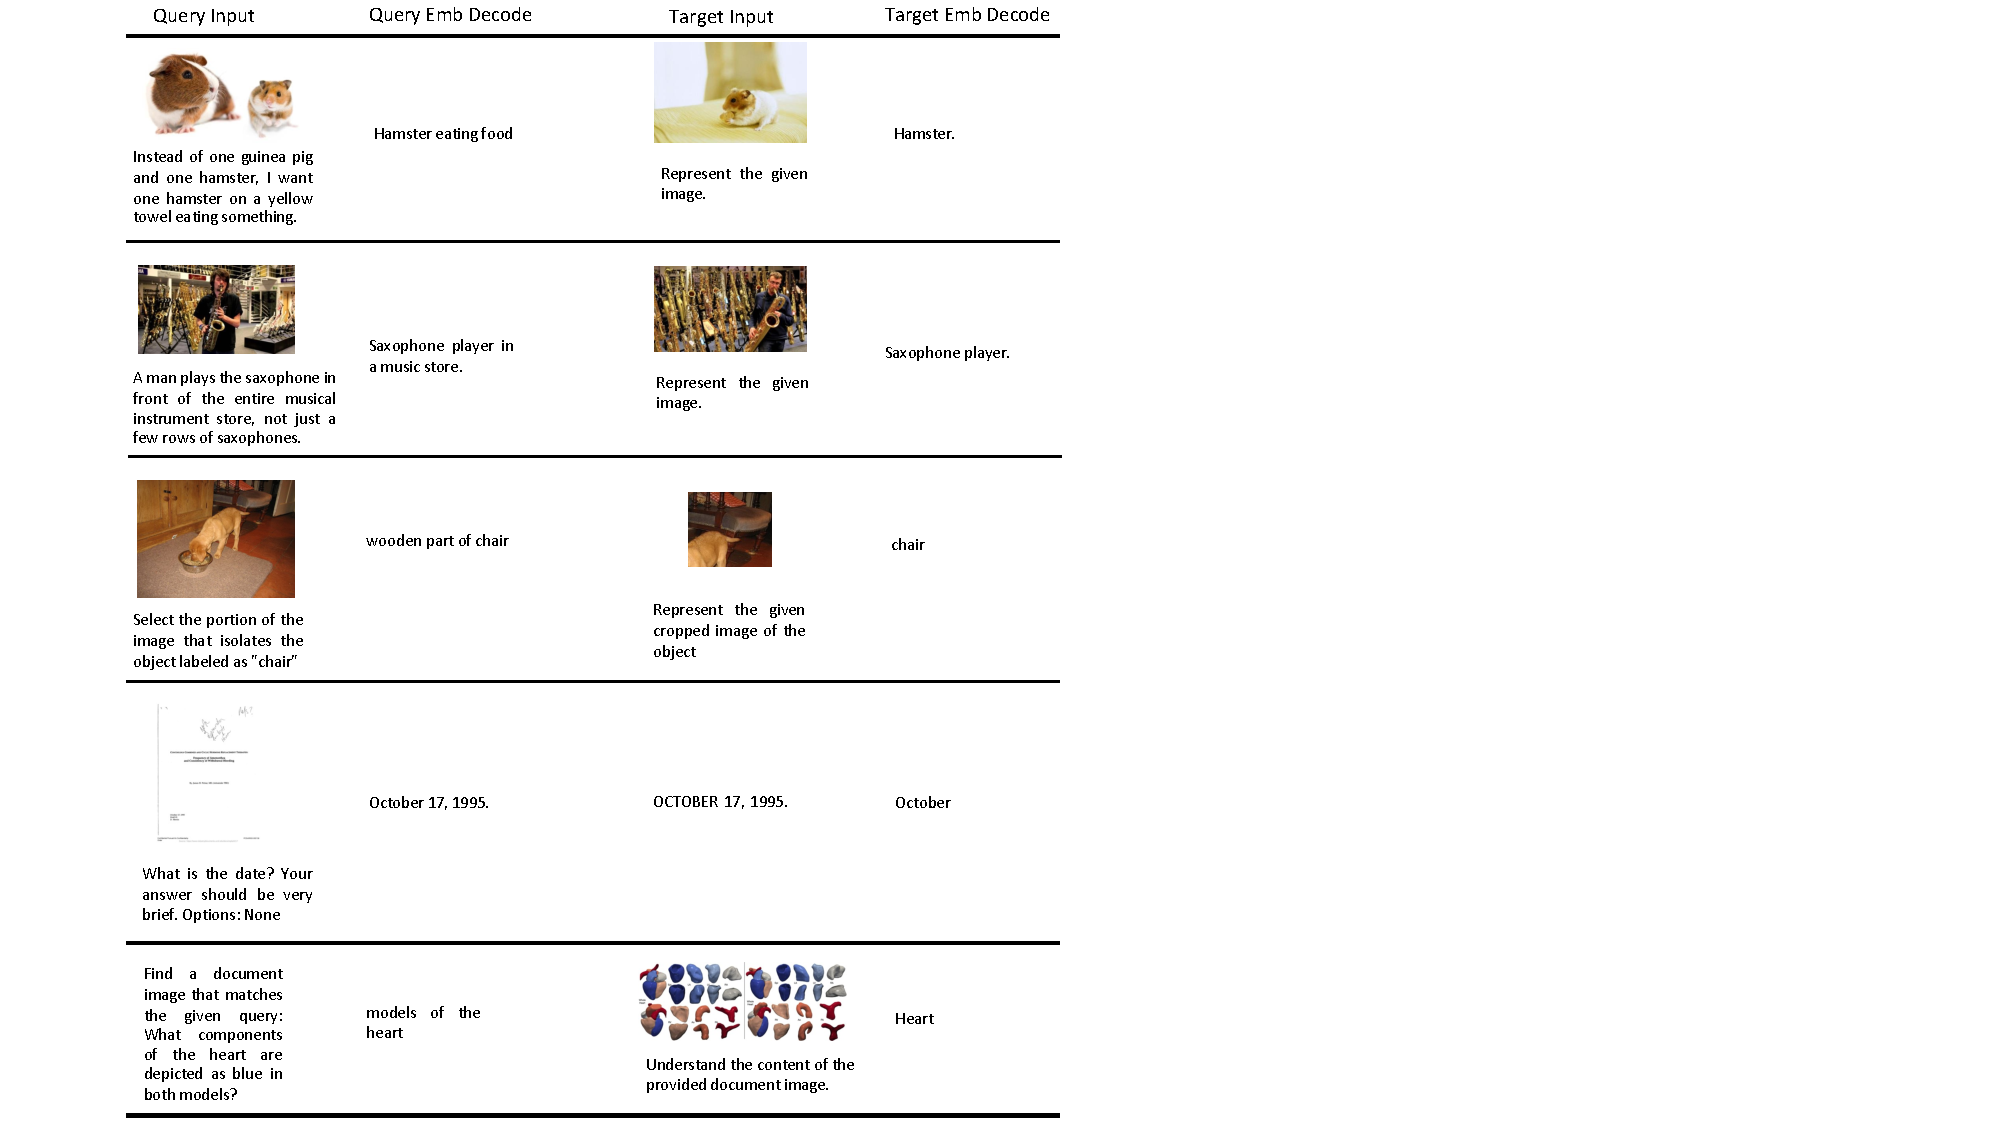
\includegraphics[width=1\linewidth]{figures/fig-generate_1.pdf}
      \caption{\textbf{Reconstruction visualization on image and visual-document inputs.}}
  \label{fig:generation_1}
\end{figure}

\begin{figure}[p]
    \centering
    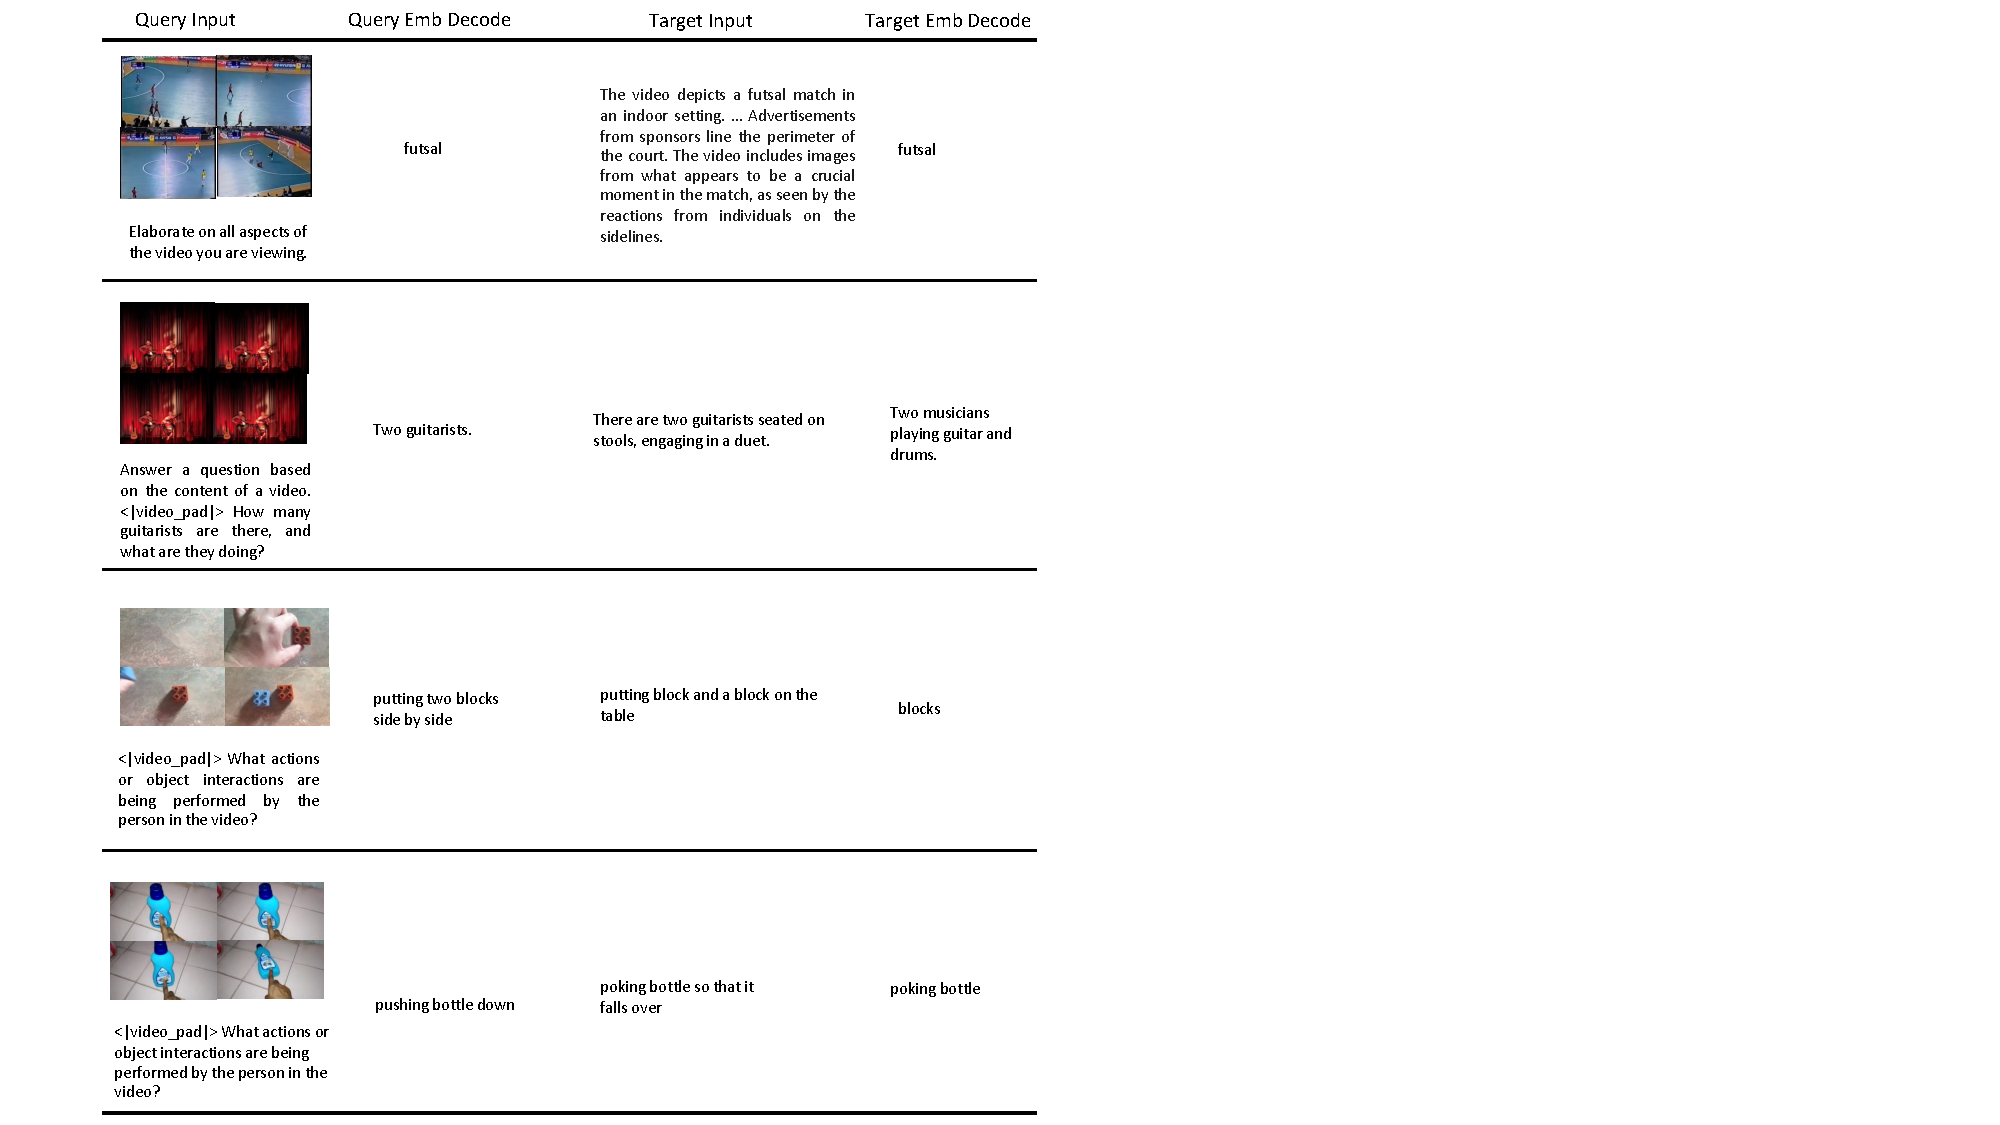
\includegraphics[width=\linewidth]{figures/fig-generate_2.pdf}
  \caption{\textbf{Reconstruction visualization on video inputs.}}
    \label{fig:generation_2}
\end{figure}

\begin{figure}[p]
    \centering
    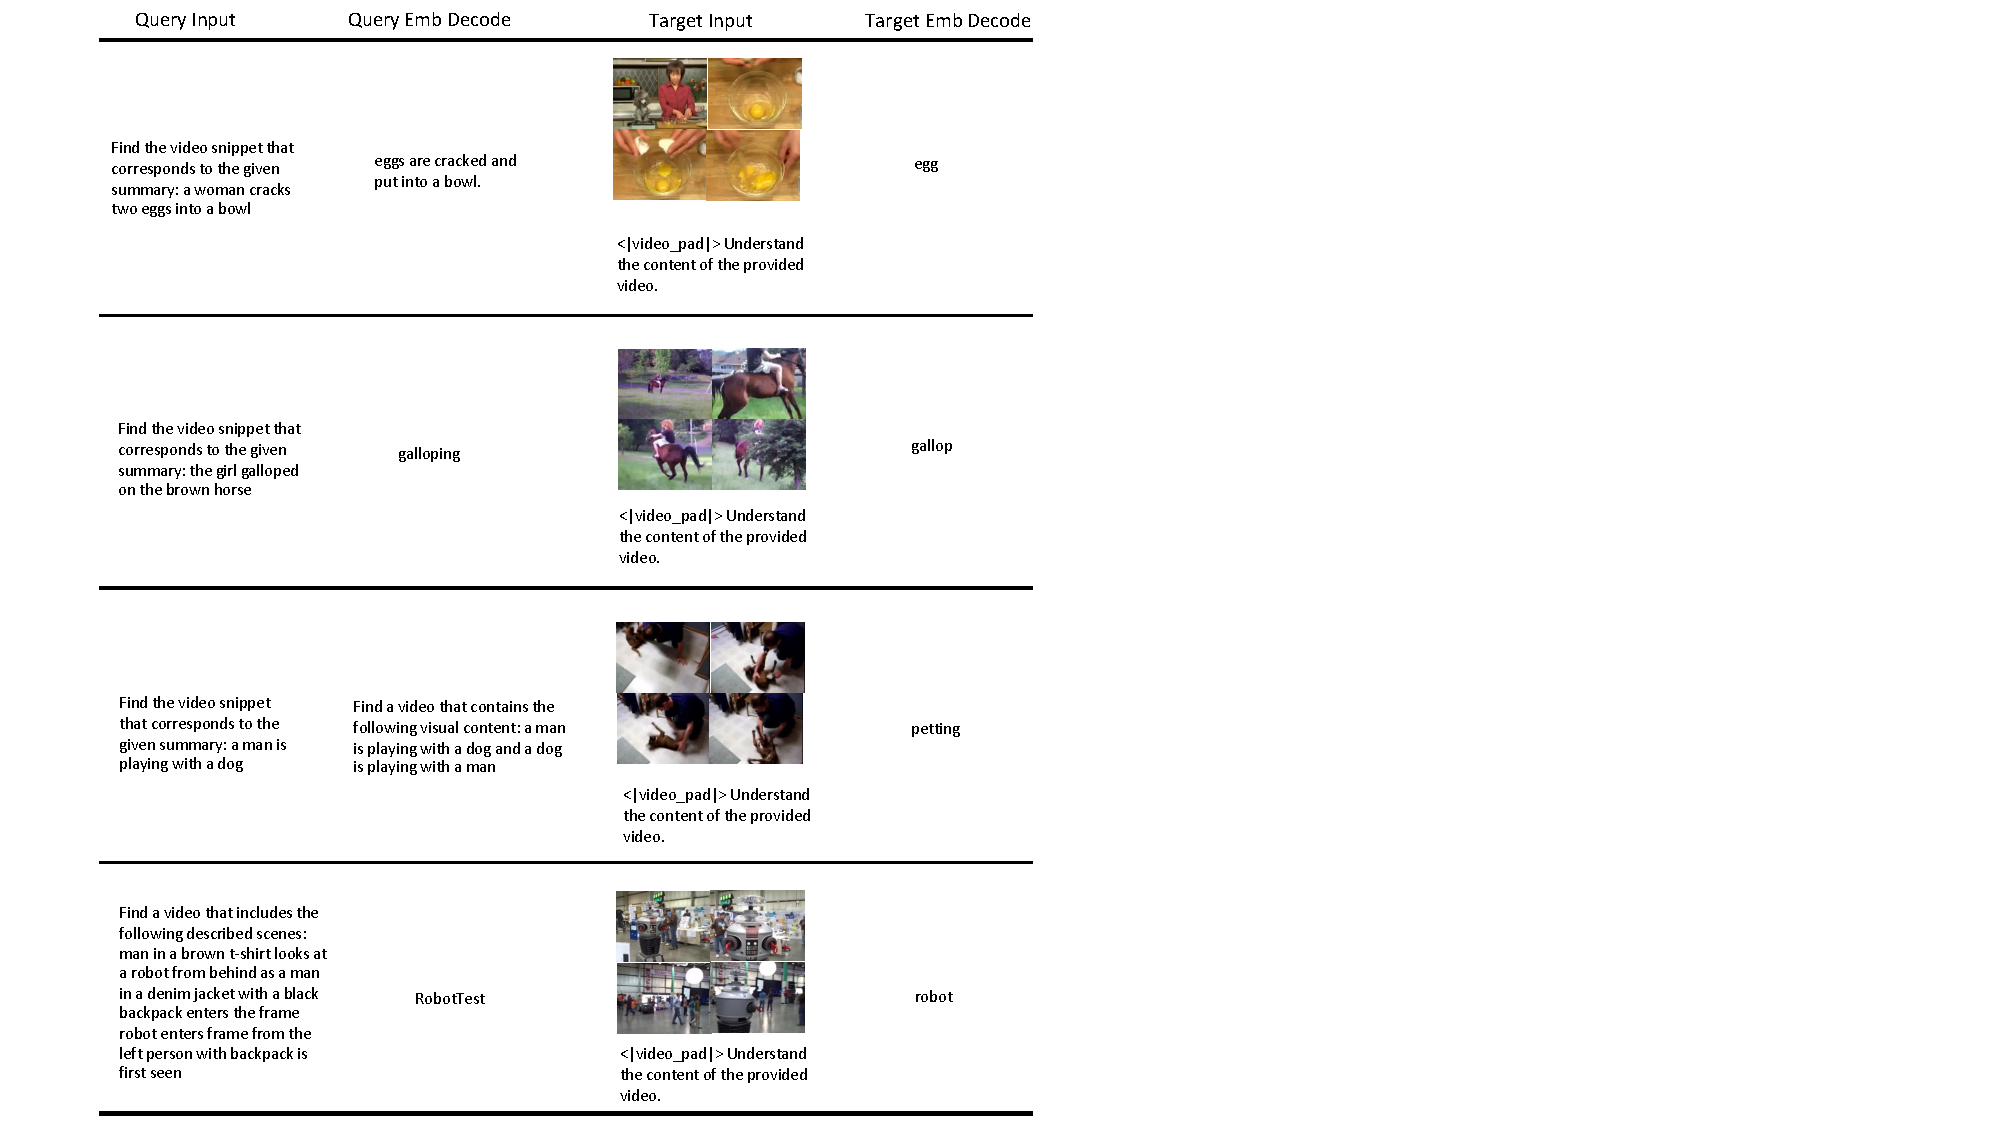
\includegraphics[width=\linewidth]{figures/fig-generate_3.pdf}
    \caption{\textbf{Reconstruction visualization on video moment-retrieval inputs.}}
    \label{fig:generation_3}
\end{figure}




